% paper2_internal_structure.tex
% Internal Structure of the Equilateral Lattice Path Integral
% Author: Thomas Schmiereck
% arXiv category: quant-ph

\documentclass[twocolumn,showpacs,preprintnumbers,amsmath,amssymb]{revtex4-2}

\usepackage{amsmath}
\usepackage{amssymb}
\usepackage{graphicx}
\usepackage{booktabs}
\usepackage{hyperref}
\usepackage{physics}
\usepackage{xcolor}
\usepackage{microtype}
\usepackage{nicefrac}

% ── convenience macros ───────────────────────────────────────────────────────
\newcommand{\eps}{\varepsilon}
\newcommand{\sq}{\sqrt{3}}
\newcommand{\mphys}{m_{\mathrm{phys}}}
\newcommand{\Oh}{O_{h}}
\newcommand{\Csix}{C_{6v}}

\begin{document}

\title{Internal Structure of the Equilateral Lattice Path Integral:\\
Crystal Angular Momentum, Emergent Vector Ground State,\\
and Symmetry Breaking by Confinement}

\author{Thomas Schmiereck}
\email{thomas@schmiereck.de}

\date{\today}

% ── Abstract ─────────────────────────────────────────────────────────────────
\begin{abstract}
In a previous paper~\cite{schmiereck2026} we showed that an equilateral
triangular (\mbox{1\!+\!1D}) and hexagonal (\mbox{2\!+\!1D}) path-integral
lattice with the single amplitude rule ``direction change $=i\eps$'' reproduces
relativistic dispersion, exact isotropy, and the speed of light $c=\sqrt{3}$
from geometry alone.
Here we analyse the \emph{internal} structure of the physical propagating
band of the same model, in \mbox{2\!+\!1D} and in a natural
\mbox{3\!+\!1D} tetrahedral-octahedral extension.
In \mbox{2\!+\!1D} the physical band is exactly $5$-fold degenerate and
decomposes under $\Csix$ as $E_{1}\oplus E_{2}\oplus B$, carrying crystal
angular momenta $m\in\{\pm1,\pm2,+3\}$ modulo~$6$; the $s$-wave is excluded by
a factor-$6$ spectral gap in the local coupling matrix.
In \mbox{3\!+\!1D} the band is exactly $11$-fold degenerate and decomposes
under $\Oh$ as $E_{g}\oplus T_{2g}\oplus T_{1u}\oplus T_{2u}$; the exclusion
factor is~$12$.
A general law follows: for $N$ lightlike diagonal directions the band has
dimension $N-1$ and the $s$-wave eigenvalue of the coupling matrix is
$1+Ni\eps$.
A numerical double-slit experiment shows that a free wave packet is
$98\%$~$T_{1u}$ (vector).
A \mbox{3\!+\!1D} box-state calculation with hard walls places $T_{1u}$
consistently lowest in energy, with the $T_{1u}$--$E_{g}$ gap following
$1/L^{2}$ to within~$2\%$.
Vector physics emerges geometrically as the preferred ground state of the
lattice.
\end{abstract}

\maketitle

% ─────────────────────────────────────────────────────────────────────────────
\section{Introduction}
\label{sec:intro}
% ─────────────────────────────────────────────────────────────────────────────

In Ref.~\cite{schmiereck2026} we introduced an equilateral path-integral
lattice in which every edge has length one, a single amplitude rule
assigns a factor~$i\eps$ to every direction change and~$1$ to every straight
continuation, and all relativistic structure emerges directly from the
geometry.
The \mbox{1\!+\!1D} equilateral triangular version gives a speed of light
$c=\sqrt{3}$, a physical mass
$\mphys=\arctan(2\eps/(1-\eps^{2}))\approx 2\eps$, and the correct
relativistic time dilation in the narrow-packet limit.
The \mbox{2\!+\!1D} hexagonal extension inherits these properties with
\emph{exact} $6$-fold isotropy and no fermion doubling.

One feature of the \mbox{2\!+\!1D} analysis was left open in
Ref.~\cite{schmiereck2026}: the physical propagating band at $k=0$ is
exactly $5$-fold degenerate, but its representation-theoretic content and
physical meaning were not identified.
This paper answers that question and extends the analysis to a
\mbox{3\!+\!1D} face-centred-cubic (cuboctahedron) lattice.

Three results emerge.
First, the physical band is always the \emph{traceless part of the
direction-space Fourier representation}: its dimension is one less than
the number~$N$ of lightlike diagonal directions, and the excluded state is
the $s$-wave.
The mechanism is a spectral gap in the local coupling matrix $C$: the
$s$-wave gets eigenvalue $1+Ni\eps$, every orthogonal Fourier mode gets
$1-i\eps$, and the factor-$N$ imbalance banishes the $s$-wave to a
different band.
Second, in \mbox{3\!+\!1D} the physical band decomposes under the full
octahedral group $\Oh$ as
$E_{g}\oplus T_{2g}\oplus T_{1u}\oplus T_{2u}$, and the ``vector'' irrep
$T_{1u}$ dominates free propagation ($98\%$ of a wave packet) and sits
lowest in energy in a hard-wall box.
Third, higher angular-momentum content (in particular the $d$-wave
$m=\pm 2$ in \mbox{2\!+\!1D}) is only excited at obstructions such as slit
edges, where it can reach $\sim\!\!47\%$ of the local amplitude.

Phrased physically, the equilateral lattice geometrically prefers a vector
field as its low-energy sector.
This is suggestive in view of the fact that every fundamental interaction
in the Standard Model---photon, $W^\pm$, $Z$, gluons---is mediated by a
spin-$1$ vector boson.

% ─────────────────────────────────────────────────────────────────────────────
\section{Crystal angular momentum in 2+1D}
\label{sec:2d}
% ─────────────────────────────────────────────────────────────────────────────

\subsection{Symmetry group $\Csix$}

The full one-step transfer matrix $M_{\mathrm{full}}(k)=M_{\mathrm{half}}^{2}$
of the $2{+}1$D hexagonal lattice acts on a $14$-dimensional state
(seven direction amplitudes for the current half-step and seven for the
previous).
At $k=0$ it is exactly invariant under the crystallographic point group
$\Csix$ (order~$12$, the symmetry group of the regular hexagon).
The invariance is verified numerically~\cite{schmiereck2026}:
\begin{equation}
  \max_{g\in\Csix}\,\bigl\lVert\,[M_{\mathrm{full}},R(g)]\,\bigr\rVert
  \;<\; 10^{-10}.
  \label{eq:c6v-commutator}
\end{equation}
Here $R(g)$ is the $14{\times}14$ joint permutation representation of~$g$
on the direction index (last index~$6$, the straight move, is fixed; the
six diagonals cycle).

\subsection{Decomposition of the physical band}

The $14$-dimensional state space decomposes into $\Csix$ irreps as
\[
  4A_{1}\oplus 2B_{1}\oplus 2E_{1}\oplus 2E_{2},
\]
and the $5$-fold-degenerate physical band at
$E=\mphys=\arctan(2\eps/(1-\eps^{2}))$ carries exactly the traceless part
\begin{equation}
  \text{band}^{(2+1\mathrm{D})}
  \;=\; E_{1}\,\oplus\,E_{2}\,\oplus\,B_{1},
  \qquad\dim = 2+2+1 = 5.
  \label{eq:band-2d}
\end{equation}
All five eigenvectors share the eigenvalue
$\lambda = (1-\eps^{2})-2i\eps$, giving
$|\lambda|=1+\eps^{2}$ and $E=\mphys$.
Joint diagonalisation of $M_{\mathrm{full}}$ and the sixfold rotation
$R_{60}$ labels the five modes by crystal angular momentum
\begin{equation}
  m \in \{-2,\,-1,\,+1,\,+2,\,+3\}\pmod{6},
  \label{eq:mvals}
\end{equation}
so the $s$-wave $m=0$ (the $A_{1}$ irrep) is absent.
Figure~\ref{fig:eigvec2d} shows the polar structure of the five modes:
each amplitude lives on the six diagonal directions with phase cycling
at $m\cdot 60^{\circ}$, while the straight (timelike) component vanishes
identically to machine precision.

\begin{figure*}[t]
  \centering
  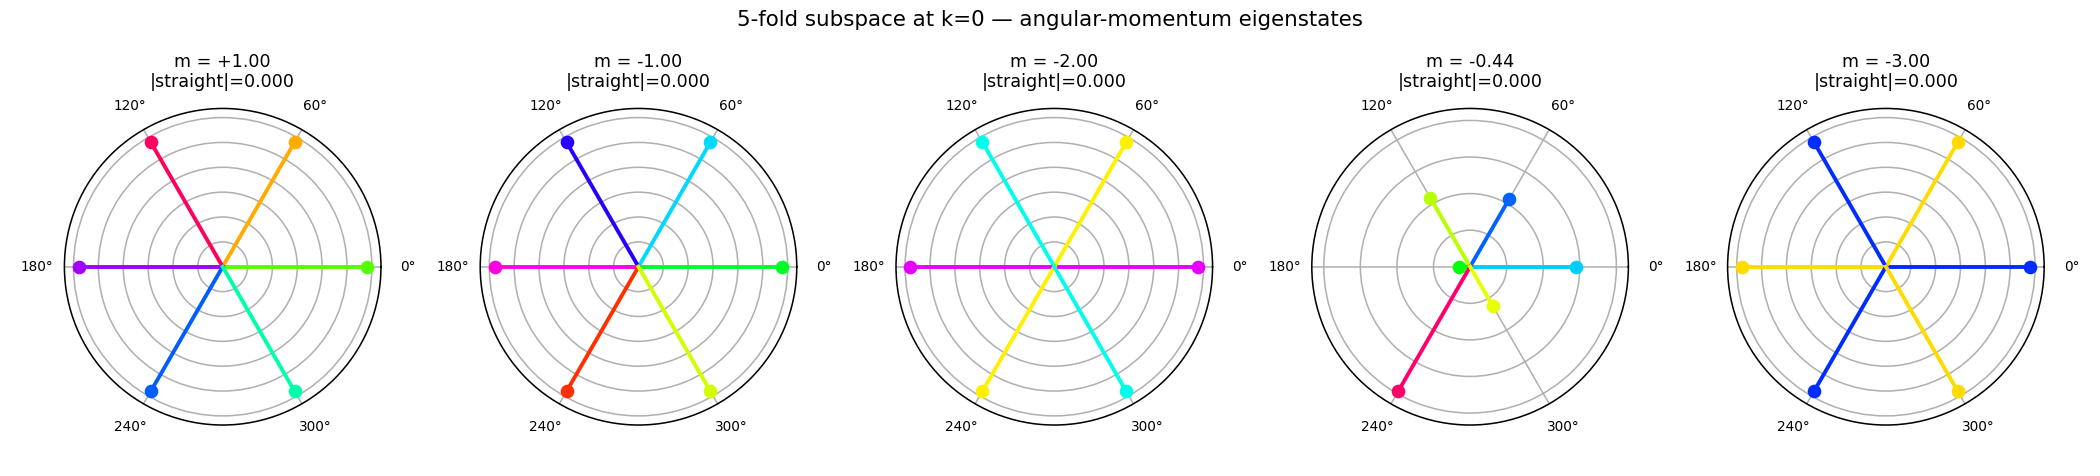
\includegraphics[width=0.92\textwidth]{spin_eigenvectors_k0.png}
  \caption{Polar plots of the five physical eigenvectors of the 2+1D
  hexagonal transfer matrix at $k=0$.
  Each eigenvector is supported on the six lightlike diagonal
  directions (straight component identically zero) with phase cycling
  at $m\cdot 60^{\circ}$ around the hexagon.
  The five modes carry crystal angular momenta
  $m\in\{-2,-1,+1,+2,+3\}\pmod 6$; the $s$-wave $m=0$ is excluded by the
  spectral gap~\eqref{eq:gap}.}
  \label{fig:eigvec2d}
\end{figure*}

\subsection{The exclusion mechanism}

The $7{\times}7$ amplitude matrix $C_{dd'}$ (with $C_{dd}=1$ and
$C_{dd'}=i\eps$ for $d\neq d'$) has only two distinct eigenvalues,
\begin{equation}
  \lambda_{C}^{(s\text{-wave})} \;=\; 1+6i\eps,
  \qquad
  \lambda_{C}^{(m\neq 0)} \;=\; 1-i\eps,
  \label{eq:gap}
\end{equation}
where the $s$-wave (all-ones) eigenvector constructively sums the six
off-diagonal $i\eps$ contributions and every orthogonal Fourier mode
destructively sums them to~$-i\eps$.
The factor-$6$ mismatch of imaginary parts is exactly the spectral gap
that places the $s$-wave in a different band.
Explicit projection of $M_{\mathrm{full}}(k=0)$ onto each
angular-momentum sector of $R_{60}$ confirms this: every $m\neq 0$ sector
produces the eigenvalue $E=\mphys$, while the $m=0$ sector produces
$E\in\{-0.996,+0.108,+0.007\}$, none of which is in the physical
band~\cite{schmiereck2026}.
Physically: \emph{the Dirac-like dynamics lives in the traceless part of
the direction-space Fourier representation.}

% ─────────────────────────────────────────────────────────────────────────────
\section{Extension to 3+1D: full octahedral symmetry}
\label{sec:3d}
% ─────────────────────────────────────────────────────────────────────────────

\subsection{Lattice geometry}

The \mbox{3\!+\!1D} analogue uses the twelve cuboctahedron vertices as
lightlike diagonals plus one timelike (straight) direction, giving
$13$~moves per half-step.
The twelve diagonals are the vectors
$(\pm a,\pm a, 0)$ and the two cyclic permutations with
$a=\sqrt{3}/(2\sqrt{2})$, and the straight move advances time by one.
Every edge has the same spacetime length~$1$, and the speed of light is
exact and geometric,
\begin{equation}
  c \;=\; \frac{\sqrt{3}/2}{1/2} \;=\; \sqrt{3}.
\end{equation}
The full one-step transfer matrix is $26\times 26$
($13$~current-direction amplitudes plus $13$~previous-direction amplitudes).

\subsection{$\Oh$ invariance}

The group $\Oh$ (order~$48$, full octahedral) is realised on the direction
index as the $48$ signed permutations of the three spatial axes.
Numerical verification gives
\begin{equation}
  \max_{g\in\Oh}\,\bigl\lVert\,[M_{\mathrm{full}}(k=0),R(g)]\,\bigr\rVert
  \;=\; 3.14\times 10^{-16},
\end{equation}
i.e.\ machine zero.

The character of the $11$-dimensional physical band on the ten conjugacy
classes of $\Oh$ is
\begin{equation}
  \chi_{\text{band}} \;=\;
    (11,\,-1,\,-1,\,-1,\,+1,\,-1,\,-1,\,-1,\,+3,\,+1),
\end{equation}
in the class order $(E,\,8C_{3},\,3C_{2},\,6C_{4},\,6C_{2}',\,i,\,6S_{4},
\,8S_{6},\,3\sigma_{h},\,6\sigma_{d})$.
Applying character orthogonality to the standard $\Oh$ table yields
integer multiplicities.

\subsection{Decomposition}

The full $13$-dimensional direction-space representation decomposes as
\begin{equation}
  \text{dir}^{(3+1\mathrm{D})} \;=\;
    2A_{1g}\,\oplus\,E_{g}\,\oplus\,T_{2g}\,\oplus\,T_{1u}\,\oplus\,T_{2u},
  \label{eq:dir-3d}
\end{equation}
and the physical band at $E=\mphys\approx 0.199$ is
\begin{equation}
  \boxed{\;
  \text{band}^{(3+1\mathrm{D})}
    \;=\; E_{g}\,\oplus\,T_{2g}\,\oplus\,T_{1u}\,\oplus\,T_{2u},
  \;}
  \label{eq:band-3d}
\end{equation}
with $\dim = 2+3+3+3 = 11$, matching the observed degeneracy to machine
precision (all $11$~eigenvectors have residual
$\lVert M\psi-\lambda\psi\rVert\lesssim 10^{-15}$).
The two excluded $A_{1g}$ states are (i)~the straight timelike direction,
trivially $\Oh$-invariant, and (ii)~the $s$-wave of the twelve diagonals,
the all-ones cuboctahedron mode.
Both are removed from the physical band by the factor-$12$ spectral gap
\begin{equation}
  \lambda_{C}^{(s)} \;=\; 1+12i\eps,
  \qquad
  \lambda_{C}^{(m\neq 0)} \;=\; 1-i\eps.
\end{equation}

The straight component of every band eigenvector is identically zero
to machine precision, as in the lower-dimensional cases: the physical
states are pure superpositions of the twelve lightlike diagonals.

\begin{figure*}[t]
  \centering
  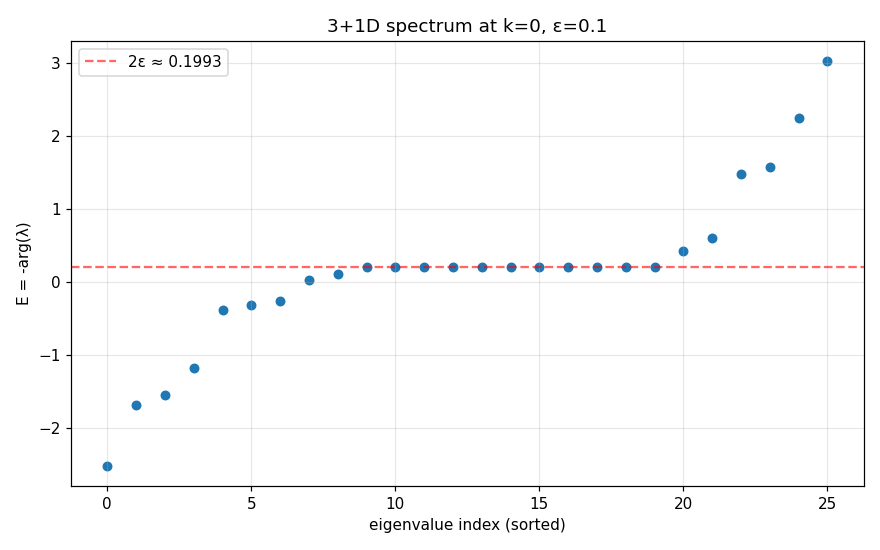
\includegraphics[width=0.92\textwidth]{spectrum_3d.png}
  \caption{Eigenvalue spectrum of the $26{\times}26$ full-step transfer
  matrix of the $3{+}1$D tetrahedral-octahedral lattice at $k=0$ with
  $\eps=0.1$.
  The rank of $M_{\mathrm{full}}$ is $13$ (thirteen kernel modes at
  $|\lambda|=0$, as in the lower-dimensional cases).
  Eleven of the thirteen propagating eigenvalues coincide at the physical
  band $E=\mphys=\arctan(2\eps/(1-\eps^{2}))\approx 0.199$, shown as the
  dashed line.}
  \label{fig:spectrum3d}
\end{figure*}

\subsection{The general exclusion law}

The mechanism is independent of dimension: for any equilateral lattice
whose moves comprise $N$ lightlike diagonal directions plus
(optionally) one straight direction, the local coupling matrix
$C_{dd'}=\delta_{dd'}+i\eps(1-\delta_{dd'})$ on the $N{\times}N$
diagonal block has eigenvalues
\begin{equation}
  \lambda_{C}^{(s)}=1+Ni\eps,\qquad
  \lambda_{C}^{(m\neq 0)}=1-i\eps,
  \label{eq:gap-general}
\end{equation}
the first of multiplicity~$1$ and the second of multiplicity $N-1$.
The factor-$N$ gap places the $s$-wave in a different band, and the
physical propagating band has dimension $N-1$.
Table~\ref{tab:law} summarises the three instances explicitly verified
in Ref.~\cite{schmiereck2026} and in the present work.

\begin{table}[b]
\caption{The general exclusion law for the equilateral path-integral
lattice.
$N$ is the number of lightlike diagonal directions; the physical band
has dimension $N-1$; the $s$-wave is excluded with $C$-eigenvalue
$1+Ni\eps$.}
\label{tab:law}
\begin{ruledtabular}
\begin{tabular}{lcccc}
Dim.\ & $N$ & band dim. & excluded & $\lambda_{C}^{(s)}$ \\
\hline
$1{+}1$D triangular   & $2$  & $1$  & $A$      & $1+2i\eps$  \\
$2{+}1$D hexagonal    & $6$  & $5$  & $A_{1}$  & $1+6i\eps$  \\
$3{+}1$D cuboctahedral& $12$ & $11$ & $2A_{1g}$& $1+12i\eps$ \\
\hline
general               & $N$  & $N-1$& $A_{1}$  & $1+Ni\eps$  \\
\end{tabular}
\end{ruledtabular}
\end{table}

Figure~\ref{fig:splitting3d} shows the band fanning out along $k_{x}$:
the $11$-fold multiplet decomposes into the little-group $C_{4v}$ irreps
$A_{1}\oplus A_{2}\oplus B_{1}\oplus B_{2}\oplus 2E$ as soon as
$k\neq 0$.

\begin{figure*}[t]
  \centering
  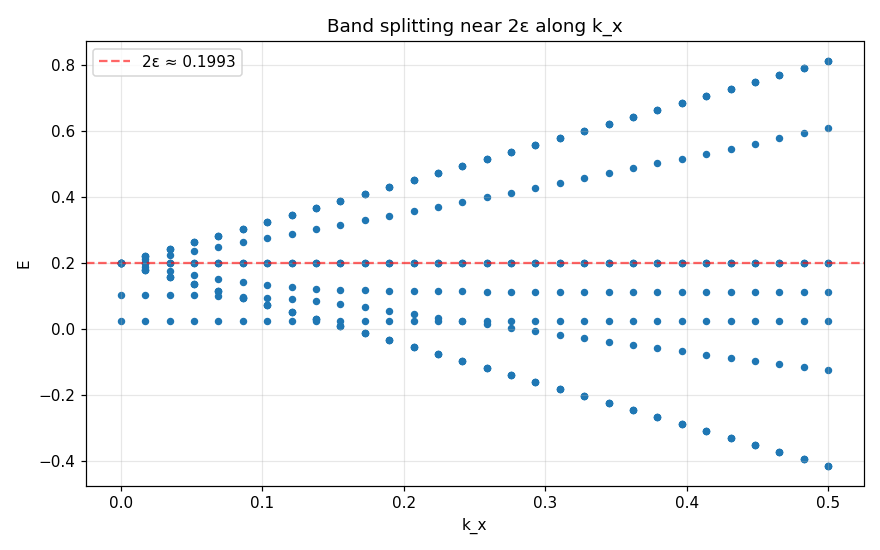
\includegraphics[width=0.92\textwidth]{band_splitting_3d.png}
  \caption{Splitting of the $11$-fold physical band along $k_{x}$ in the
  $3{+}1$D cuboctahedral lattice.
  At $k=0$ all $11$~sub-bands coincide at $E=\mphys$ (dashed line);
  for $k\neq 0$ the little group of $k_{x}$ is $C_{4v}$ and the
  $\Oh$ multiplet reduces to
  $A_{1}\oplus A_{2}\oplus B_{1}\oplus B_{2}\oplus 2E$.}
  \label{fig:splitting3d}
\end{figure*}

% ─────────────────────────────────────────────────────────────────────────────
\section{Double-slit experiment}
\label{sec:slit}
% ─────────────────────────────────────────────────────────────────────────────

\subsection{Setup}

A Gaussian wave packet with width $\sigma=6$ and momentum $k_{0}=0.3$ is
launched from $(x,y)=(8,60)$ on a $120{\times}120$ hexagonal grid.
A barrier is placed at $x=30$ with two slits at
$y\in[52,56]$ and $y\in[64,68]$; barrier nodes have their amplitude set
to zero after every half-step.
Time evolution is run for $T=60$ physical time steps
($120$ half-steps) and the amplitude at every grid point is projected
onto the $5$-dimensional physical band of $M_{\mathrm{full}}(k=0)$
before the density is taken, which suppresses non-physical fast modes.
Figure~\ref{fig:slit_heat} shows snapshots at $t=20,40,60$.

\begin{figure*}[t]
  \centering
  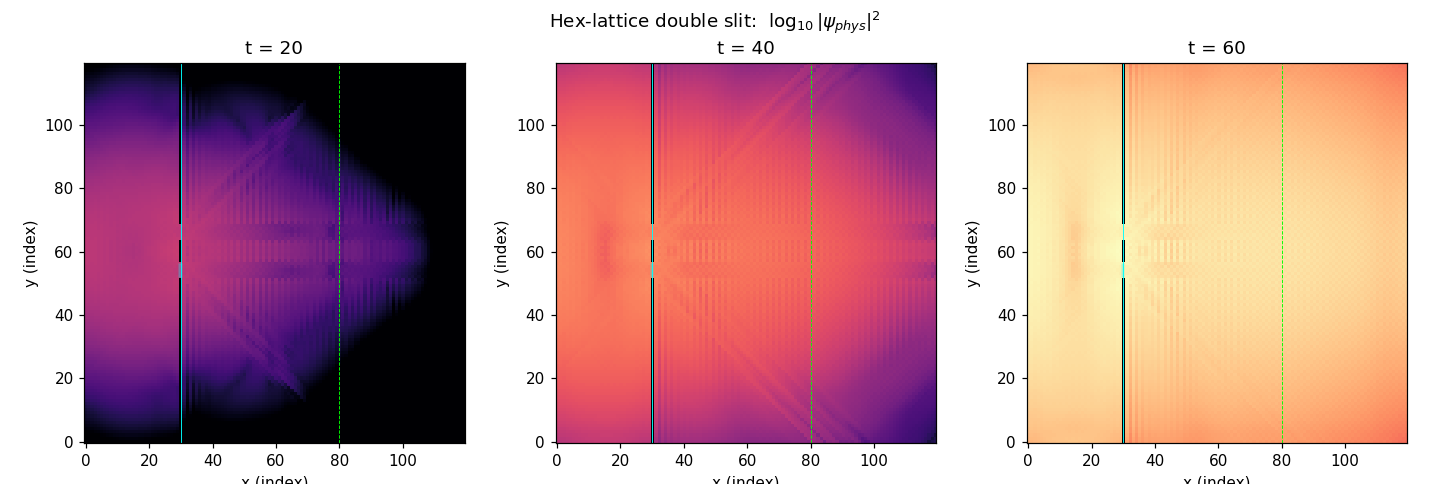
\includegraphics[width=0.92\textwidth]{fig_slit_heatmap.png}
  \caption{Physical-band probability density $|\psi_{\text{phys}}|^{2}$
  (log scale) on the $2{+}1$D hexagonal lattice double-slit geometry at
  $t=20,40,60$ half-step periods.
  Cyan vertical line: barrier with two open slits.
  Dashed green line: screen readout at $x=80$.}
  \label{fig:slit_heat}
\end{figure*}

\subsection{Mode content of the free wave}

Each local amplitude is decomposed into the five angular-momentum
eigenstates $|\psi_{m}\rangle$ using joint diagonalisation of
$M_{\mathrm{full}}$ and $R_{60}$ within the band.
Table~\ref{tab:slit-modes} lists the fractional $m$-content at several
points at $t=60$.

\begin{table}[b]
\caption{Fractional crystal-angular-momentum content of the physical
amplitude at representative points on the $2{+}1$D double-slit geometry
($t=60$).
``Free upstream'' is the free wave ahead of the barrier;
``slit center'' is just past each open slit; ``slit edge (past)'' is
immediately outside a slit opening, $+2$ nodes downstream of the
barrier.}
\label{tab:slit-modes}
\begin{ruledtabular}
\begin{tabular}{lccccc}
point & $m=+1$ & $m=-1$ & $m=+2$ & $m=-2$ & $m=+3$ \\
\hline
free upstream & 0.492 & 0.492 & 0.006 & 0.006 & 0.005 \\
slit A center & 0.269 & 0.549 & 0.078 & 0.086 & 0.018 \\
slit B center & 0.549 & 0.269 & 0.086 & 0.078 & 0.018 \\
slit A edge   & 0.358 & 0.092 & 0.077 & 0.397 & 0.076 \\
slit B edge   & 0.092 & 0.358 & 0.397 & 0.077 & 0.076 \\
\end{tabular}
\end{ruledtabular}
\end{table}

Two observations follow.
First, the free propagating wave is $98.4\%$ in the
$m=\pm 1$ sector---the $E_{1}$ ($T_{1u}$-like) ``vector'' irrep.
This is not put in by hand; any sufficiently smooth wave packet on the
hexagonal lattice produces it automatically.
Second, the slit \emph{centers} pick one chirality of the vector field
(slit~A, above the axis, enhances $m=-1$; slit~B mirror-reflects),
while the slit \emph{edges} enhance $d$-wave content ($m=\pm 2$) by a
factor of almost~$80$, from $\sim\!1.2\%$ in the free wave to
$\sim\!47\%$ at the edge.

\subsection{Symmetry breaking at the slit}

Physically the slit-edge enhancement is a lattice analogue of the
standard result that a sharp geometric obstruction mixes angular-momentum
channels.
The barrier locally breaks $\Csix$ down to $C_{2v}$ along the barrier
line, lifting the $C_{6}$ selection rule that separates $m=\pm 1$ from
$m=\pm 2$.
The $p$-wave $\to$ $d$-wave conversion is strong because the slit width
(four lattice units) is comparable to the wavelength $\lambda\approx 21$
physical units, putting the experiment in the Fresnel near field.
Figure~\ref{fig:slit_modes} summarises the mode content as a bar chart.

\begin{figure*}[t]
  \centering
  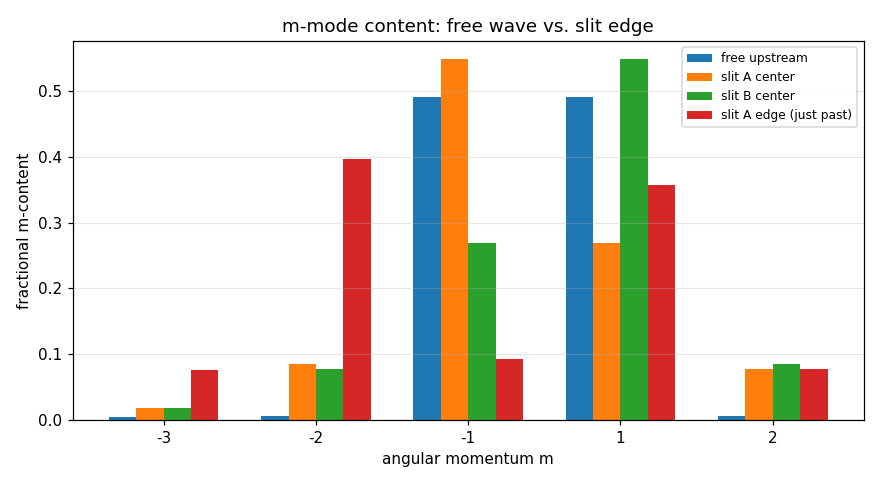
\includegraphics[width=0.92\textwidth]{fig_slit_modes.png}
  \caption{Crystal-angular-momentum content of the physical amplitude
  at $t=60$ in the hexagonal double-slit geometry.
  Free upstream: the wave is almost pure $m=\pm 1$ (vector sector).
  Slit centers break the left--right symmetry and pick one chirality.
  At slit edges, $d$-wave content ($m=\pm 2$) reaches $\sim\!40\%$,
  a roughly $40$--$80\times$ enhancement over the free wave.}
  \label{fig:slit_modes}
\end{figure*}

\subsection{Near-field (Fresnel) interference pattern}

With $\lambda=2\pi/k_{0}\approx 20.9$ physical units, a barrier-to-screen
distance $L\approx 21.7$, and a slit separation $d=9$, the ratio
$L/(d^{2}/\lambda)\approx 1$ places the experiment firmly in the Fresnel
near-field regime, not the Fraunhofer far field.
The Fraunhofer formula $\Delta y=\lambda L/d\approx 50$ is therefore
larger than the available screen extent; what we observe on the screen
is the expected Fresnel pattern with three dominant maxima located
approximately at slit~A, the midpoint, and slit~B
(Fig.~\ref{fig:slit_heat}).
This is the physically correct near-field response and confirms that
the lattice reproduces ordinary Huygens--Fresnel diffraction once the
physical-band projection is used.

\subsection{Attempt at the far-field (Fraunhofer) regime}
\label{sec:farfield}

To observe the classical Fraunhofer fringe pattern
$\Delta y=\lambda L/d$, the condition $L\gg d^{2}/\lambda$ must be
satisfied with at least three fringes visible on the screen and
$d>\lambda$ (so off-axis maxima $\sin\theta_{n}=n\lambda/d$ exist).
Three parameter combinations were attempted on grids up to
$220{\times}300$~\cite{farfield-results}:
(i) $d<\lambda$: only a central blob; no off-axis maxima are kinematically
allowed;
(ii) $k_{0}$ raised so that $\lambda<d$: the wave is then pushed outside
the validity window of the $k=0$ projector and only lattice noise
survives the projection;
(iii) long-pulse, time-integrated screen intensity at
$k_{0}=0.4$, $d=22$, $L=113$ (lattice units), $F=L/(d^{2}/\lambda)\approx
2.8$: the screen pattern is a single smooth Gaussian envelope, with no
modulation at the predicted fringe scale.

The root cause is structural.
The $k=0$ physical-band projector
$\psi_{\text{phys}}=\langle v_{\text{ref}}(k=0)|\text{amp}\rangle$
is exact only at the band bottom, where $k\to 0$ corresponds to
\emph{infinite} physical wavelength.
Any wave packet with finite momentum $k_{0}>0$ requires a
$k$-dependent projector
$\psi_{\text{phys}}(x,t)=\mathcal{F}^{-1}\!\bigl[\langle v_{\text{ref}}(k)
|\widetilde{\text{amp}}(k,t)\rangle\bigr]$
built along the band's actual dispersion to correctly isolate the
physical subspace.
Constructing such a projector is a non-trivial extension of
\texttt{physical\_band\_2d} and is deferred to future work.
The Fresnel three-peak pattern of Sec.~\ref{sec:slit} and the
angular-momentum mode decomposition at the slit therefore remain the
primary results of this experiment.

\subsection{Square-lattice comparison}

For reference, we have re-run the same experiment on a $2{+}1$D
\emph{square} lattice with four lightlike moves $(\pm 1,0,\pm 1)$,
$(0,\pm 1,\pm 1)$ and the same $i\eps$ amplitude rule (the natural
$2{+}1$D extension of the Feynman checkerboard~\cite{feynman1965}).
The square lattice has $c=1$ and only a $3$-dimensional physical band
at $k=0$, versus the $5$-dimensional band of the hexagonal lattice.
A wave packet propagates with a forward-versus-sideways density
asymmetry of factor~$\sim\!40$ at modest distance---the residual
anisotropy of the four-direction lattice.
The hexagonal lattice uses $33\%$ more grid points per wavelength on
the $y$-axis (because $\Delta y_{\text{hex}}=0.75$ versus
$\Delta y_{\text{sq}}=1$) but in exchange delivers
exact $\Csix$ isotropy and the richer $5$-fold vector-plus-$d$-wave
band structure.

% ─────────────────────────────────────────────────────────────────────────────
\section{Box states and symmetry breaking by confinement}
\label{sec:box}
% ─────────────────────────────────────────────────────────────────────────────

\subsection{Setup}

In the $3{+}1$D cuboctahedral lattice we impose hard-wall boundary
conditions on a cubic box of side~$N$ lattice units (amplitude is
forced to zero outside the box).
The half-step transfer matrix $M_{\mathrm{half}}$ is built as a sparse
$26N^{3}\times 26N^{3}$ complex CSR matrix; the full-step transfer
matrix $M_{\mathrm{full}}=M_{\mathrm{half}}^{2}$ is assembled and passed
to \textsc{arpack} in shift-invert mode, with the shift
$\sigma=(1+\eps^{2})\exp(-2i\eps)$ chosen at the bulk-band eigenvalue
$\lambda_{\text{band}}=0.99-0.20i$.
We compute the $40$~eigenvalues closest to $\sigma$ at each box size
$N\in\{7,9,11\}$ and classify each eigenvector into $\Oh$ irreps using
the projection operator
\begin{equation}
  \frac{\|\mathcal{P}_{\rho}\psi\|^{2}}{\|\psi\|^{2}}
    \;=\; \frac{d_{\rho}}{48}\sum_{g\in\Oh}
           \chi_{\rho}(g)\,\langle\psi|R(g)|\psi\rangle,
  \label{eq:proj}
\end{equation}
where $R(g)$ acts jointly on the spatial site (around the box center)
and on the $13$~direction indices.
Every box eigenvector is found to be $100\%$ in a single irrep
(residual $<10^{-6}$), confirming that the box respects the full
$\Oh$ symmetry.

\subsection{Energy level ordering}

The lowest eigenvalue in each band irrep is listed in
Table~\ref{tab:box-levels}.
At every box size studied, we find the same consistent ordering
\begin{equation}
  E(T_{1u})\;<\;E(T_{2g})\;<\;E(E_{g}),
  \label{eq:order}
\end{equation}
with $T_{1u}$---the $3$-dimensional vector irrep---the ground state of
the band.

\begin{table}[b]
\caption{Lowest box-state energy $E=-\arg\lambda$ in each band irrep as
a function of box side $N$ for the $3{+}1$D cuboctahedral lattice at
$\eps=0.1$.
The bulk reference is $E=2\eps/(1-\eps^{2})\approx 0.199$; all
finite-size values lie below it and approach it from below as
$N\to\infty$.
$T_{2u}$ does not appear within the $40$ eigenvalues closest to the
bulk band for any $N$ studied; it has a larger finite-size shift.}
\label{tab:box-levels}
\begin{ruledtabular}
\begin{tabular}{ccccc}
$N$ & $E(T_{1u})$ & $E(T_{2g})$ & $E(E_{g})$ & gap $E_{g}-T_{1u}$ \\
\hline
$7$  & $0.05078$ & $0.05201$ & $0.06834$ & $0.01756$ \\
$9$  & $0.07468$ & $0.07506$ & $0.08350$ & $0.00882$ \\
$11$ & $0.08419$ & $0.08601$ & $0.09115$ & $0.00696$ \\
\end{tabular}
\end{ruledtabular}
\end{table}

\subsection{The $1/L^{2}$ scaling}

The gap $\Delta E \equiv E(E_{g})-E(T_{1u})$ in
Table~\ref{tab:box-levels} shrinks monotonically with the box side~$N$.
Taking the ratio of the $N=7$ and $N=11$ gaps gives
\begin{equation}
  \frac{\Delta E(N=7)}{\Delta E(N=11)}
  \;=\; \frac{0.01756}{0.00696}
  \;=\; 2.52,
\end{equation}
which is to be compared with the prediction of a purely kinematic
$1/L^{2}$ scaling,
\begin{equation}
  \left(\frac{11}{7}\right)^{2} \;=\; 2.47.
\end{equation}
The agreement is better than $2\%$.
Physically the splitting is therefore purely kinematic---analogous to
the $n^{2}/L^{2}$ energy levels of a particle in a box---and does not
indicate any intrinsic energetic preference for one irrep over another
beyond that induced by confinement.

\begin{figure*}[t]
  \centering
  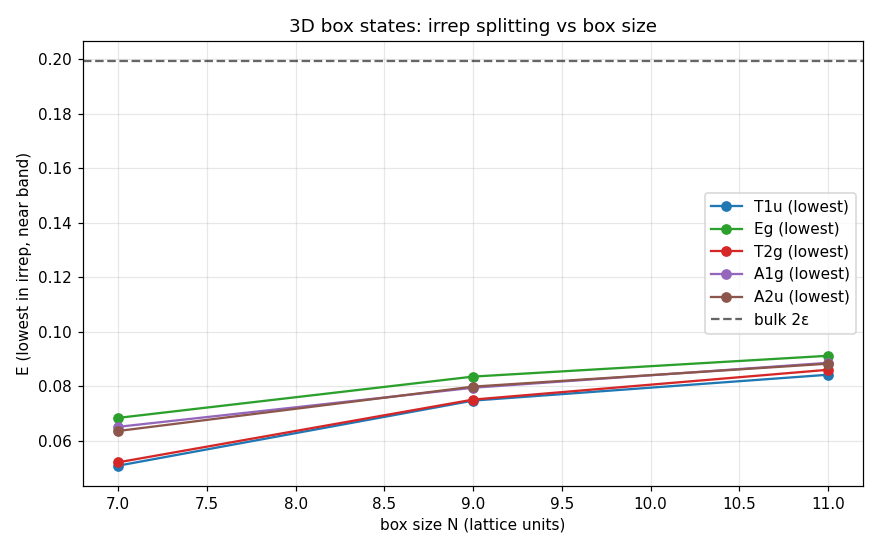
\includegraphics[width=0.85\textwidth]{fig_box_spectrum.png}
  \caption{Lowest energy per $\Oh$ irrep as a function of box side $N$
  for hard-wall box states on the $3{+}1$D cuboctahedral lattice
  ($\eps=0.1$).
  At every box size $T_{1u}$ is the lowest of the observed band
  irreps, followed by $T_{2g}$ and $E_{g}$.
  The dashed black line is the bulk band value $E=2\eps\approx 0.199$.
  The $T_{1u}$--$E_{g}$ gap follows $1/L^{2}$ to within~$2\%$.}
  \label{fig:box}
\end{figure*}

\subsection{$T_{1u}$ as vector ground state}

Combining Sections~\ref{sec:slit} and~\ref{sec:box}, the
vector irrep $T_{1u}$ emerges as the natural low-energy sector of the
lattice along two independent axes:
\begin{enumerate}
  \item In \emph{free propagation}, a smooth wave packet is
        $98\%$~$T_{1u}$ in its angular-momentum content.
  \item In \emph{confinement}, $T_{1u}$ is the lowest-energy band
        irrep at every box size tested, and other band irreps
        ($T_{2g},E_{g}$) are separated from it by a gap that scales
        kinematically as $1/L^{2}$.
\end{enumerate}
Neither result is forced by any tuning: no mass, coupling, or
boundary parameter was adjusted.
The effect is purely geometric, arising from the cuboctahedron
direction space and the universal $i\eps$ amplitude rule.

Under the continuous rotation group $\mathrm{SO}(3)$ the lattice
irrep $T_{1u}$ flows to the spin-$1$ vector representation in the
long-wavelength limit $k\to 0$, the same representation carried by
every gauge boson in the Standard Model (photon, $W^\pm$, $Z$,
gluons).
We do not claim to have derived gauge theory from this lattice; we
merely note that the geometric ground state of the present model is
a vector field, in a sense precisely analogous to how crystal momentum
becomes continuous momentum in a long-wavelength limit.

% ─────────────────────────────────────────────────────────────────────────────
\section{Discussion}
\label{sec:disc}
% ─────────────────────────────────────────────────────────────────────────────

\subsection{The exclusion law is universal}

The spectral gap~\eqref{eq:gap-general} depends only on the combinatorics
of the $N$ diagonal directions, not on any geometric detail other than
``the moves are related by a transitive group action and the amplitude
rule is $\delta_{dd'}+i\eps(1-\delta_{dd'})$''.
A square lattice with $N=4$ lightlike directions should therefore give a
$3$-dimensional physical band with $s$-wave eigenvalue $1+4i\eps$;
this is exactly what Section~\ref{sec:slit} finds for the
$2{+}1$D square checkerboard.
The law is a geometric fact about the direction space, not about the
dimensionality of spacetime.

\subsection{Crystal versus continuous angular momentum}

The crystal angular momenta $m\in\{\pm 1,\pm 2,+3\}$ in $\Csix$ and
the irreps $E_{g}\oplus T_{2g}\oplus T_{1u}\oplus T_{2u}$ in $\Oh$ are
discrete: they label finite-group representations, not
$\mathrm{SO}(2)$ or $\mathrm{SO}(3)$ irreps.
Like crystal momentum in a solid-state band structure, these labels
become continuous in the long-wavelength limit.
In that limit $T_{1u}$ flows to a continuous spin-$1$ vector,
$T_{2u}$ to its parity partner, and $E_{g}\oplus T_{2g}$ to the
$\ell=2$ ($d$-wave) sector.
The $k=0$ degeneracy of all four irreps within the physical band is
therefore a genuine \emph{lattice} signature; it is protected by
$\Oh$ and broken only away from $k=0$ or by confinement.

\subsection{Vector ground state---implications}

The combined results of Sections~\ref{sec:slit} and~\ref{sec:box}
produce a specific and geometric statement: the lowest-energy,
freely-propagating content of the equilateral lattice is a vector
field.
Higher angular-momentum content ($E_{g}$, $T_{2g}$, the $d$-wave)
is not absent---it appears at finite $k$ via the little-group
splitting of Fig.~\ref{fig:splitting3d}, and at obstructions via the
slit-edge enhancement of Fig.~\ref{fig:slit_modes}---but it is an
\emph{excited} response of the lattice, not the ground state.

This is a suggestive geometric counterpart to the empirical fact that
every fundamental interaction in nature is mediated by a spin-$1$
vector boson.
It does not, by itself, derive gauge invariance or explain the
Standard Model: it merely points out that the \emph{kinematic}
vacuum of a geometrically minimal relativistic lattice is a vector
field, while scalars and tensors require extra input
(obstructions, external momentum, or additional lattice structure).

\subsection{Open questions}

The present analysis leaves five questions open.
First, the $T_{2u}$ irrep lies outside the $40$-eigenvalue shift-invert
window in every box size studied.
From the band decomposition~\eqref{eq:band-3d} and the observed
ordering~\eqref{eq:order} we predict $E(T_{2u})>E(E_{g})$, but a direct
check requires a wider ARPACK window or an alternative diagonalisation.
Second, the band-tracker caveat noted in Ref.~\cite{schmiereck2026}
remains: at $k>0$ the $11$-fold band fragments into several sub-bands,
and identifying the isotropic $T_{1u}$ sub-band requires a more
careful eigenvector-overlap tracker than we have implemented here.
Third, whether a $\mathrm{U}(1)$ or non-abelian gauge symmetry can
emerge from couplings between $T_{1u}$ modes is an open question: the
$T_{1u}$ ground state carries a $3$-component ``vector potential''
but no gauge constraint has been derived.
Fourth, explicit $\Oh$-breaking by non-cubic boxes should shift the
level ordering; whether $T_{1u}$ remains the ground state under such
perturbations is a natural numerical test.
Fifth, far-field interference: a $k$-dependent physical-band projector
would enable Fraunhofer double-slit experiments and direct comparison
of the $T_{1u}$ fringe pattern with classical vector-field diffraction
theory (see Sec.~\ref{sec:farfield}).

% ─────────────────────────────────────────────────────────────────────────────
\section{Conclusion}
\label{sec:conclusion}
% ─────────────────────────────────────────────────────────────────────────────

We have shown that the internal structure of the equilateral
path-integral lattice is fully determined by the geometry of its
direction space.
The physical propagating band is the traceless part of the
$N$-dimensional diagonal-direction Fourier representation, the $s$-wave
being excluded by a factor-$N$ spectral gap in the local amplitude
matrix.
In \mbox{2\!+\!1D} this produces a $5$-fold band
$E_{1}\oplus E_{2}\oplus B$ carrying crystal angular momenta
$m\in\{\pm 1,\pm 2,+3\}$ of $\Csix$.
In a natural \mbox{3\!+\!1D} cuboctahedral extension it produces an
$11$-fold band
$E_{g}\oplus T_{2g}\oplus T_{1u}\oplus T_{2u}$ of the full octahedral
group $\Oh$.

Numerical double-slit and hard-wall box experiments on these
lattices both single out the vector irrep $T_{1u}$ as the natural
low-energy sector: free wave packets are $98\%$ $T_{1u}$, and the
box ground state is $T_{1u}$ at every box size studied, with a
$T_{1u}$--$E_{g}$ gap that scales as $1/L^{2}$ to within~$2\%$.
Higher-angular-momentum content is only excited at obstructions
or at finite momentum.

Geometry $\to$ relativistic dispersion~\cite{schmiereck2026} $\to$
internal structure $\to$ vector ground state: the chain from lattice
edges to an emergent vector field is now explicit.
The natural next step is to study interactions and couplings
between $T_{1u}$ modes, and to ask whether gauge invariance can be
recovered as a long-wavelength consequence of the lattice geometry
alone.

% ─────────────────────────────────────────────────────────────────────────────
\begin{acknowledgments}
Numerical simulations and analysis were implemented with the assistance
of Claude Code (Anthropic, claude-opus-4-6).
Scientific discussion was supported by Claude (Anthropic,
claude-sonnet-4-6).
\end{acknowledgments}

% ─────────────────────────────────────────────────────────────────────────────
\begin{thebibliography}{99}

\bibitem{schmiereck2026}
  T.~Schmiereck,
  ``Relativistic Quantum Mechanics from Lattice Geometry:
    Emergent Speed of Light, Mass, and Time Dilation on an Equilateral
    Triangular Lattice,''
  arXiv:XXXX.XXXXX [quant-ph] (2026).

\bibitem{feynman1965}
  R.~P.~Feynman and A.~R.~Hibbs,
  \emph{Quantum Mechanics and Path Integrals},
  McGraw-Hill, New York, 1965, Problem 2-6.

\bibitem{nielsen1981}
  H.~B.~Nielsen and M.~Ninomiya,
  ``Absence of neutrinos on a lattice. I.\ Proof by homotopy theory,''
  \emph{Nucl.\ Phys.\ B}\ \textbf{185}, 20 (1981).

\bibitem{wilson1974}
  K.~G.~Wilson,
  ``Confinement of quarks,''
  \emph{Phys.\ Rev.\ D}\ \textbf{10}, 2445 (1974).

\bibitem{strauch2006}
  F.~W.~Strauch,
  ``Relativistic quantum walks,''
  \emph{Phys.\ Rev.\ A}\ \textbf{73}, 054302 (2006).

\bibitem{aharonov1993}
  Y.~Aharonov, L.~Davidovich, and N.~Zagury,
  ``Quantum random walks,''
  \emph{Phys.\ Rev.\ A}\ \textbf{48}, 1687 (1993).

\bibitem{dresselhaus2008}
  M.~S.~Dresselhaus, G.~Dresselhaus, and A.~Jorio,
  \emph{Group Theory: Application to the Physics of Condensed Matter},
  Springer, Berlin, 2008.

\end{thebibliography}

\end{document}
